\documentclass{article}

\usepackage{graphicx}
\usepackage{tikz}
\usepackage{tikzsymbols}
\usetikzlibrary{calc,patterns,shapes.geometric}
\pagestyle{empty}
\usepackage[margin=0pt]{geometry}
\geometry{papersize={14in,12in}}

\def\centerarc[#1](#2)(#3:#4:#5){\draw[#1] ($(#2)+({#5*cos(#3)},{#5*sin(#3)})$) arc (#3:#4:#5);}

\begin{document}
	\begin{figure}
		\centering
		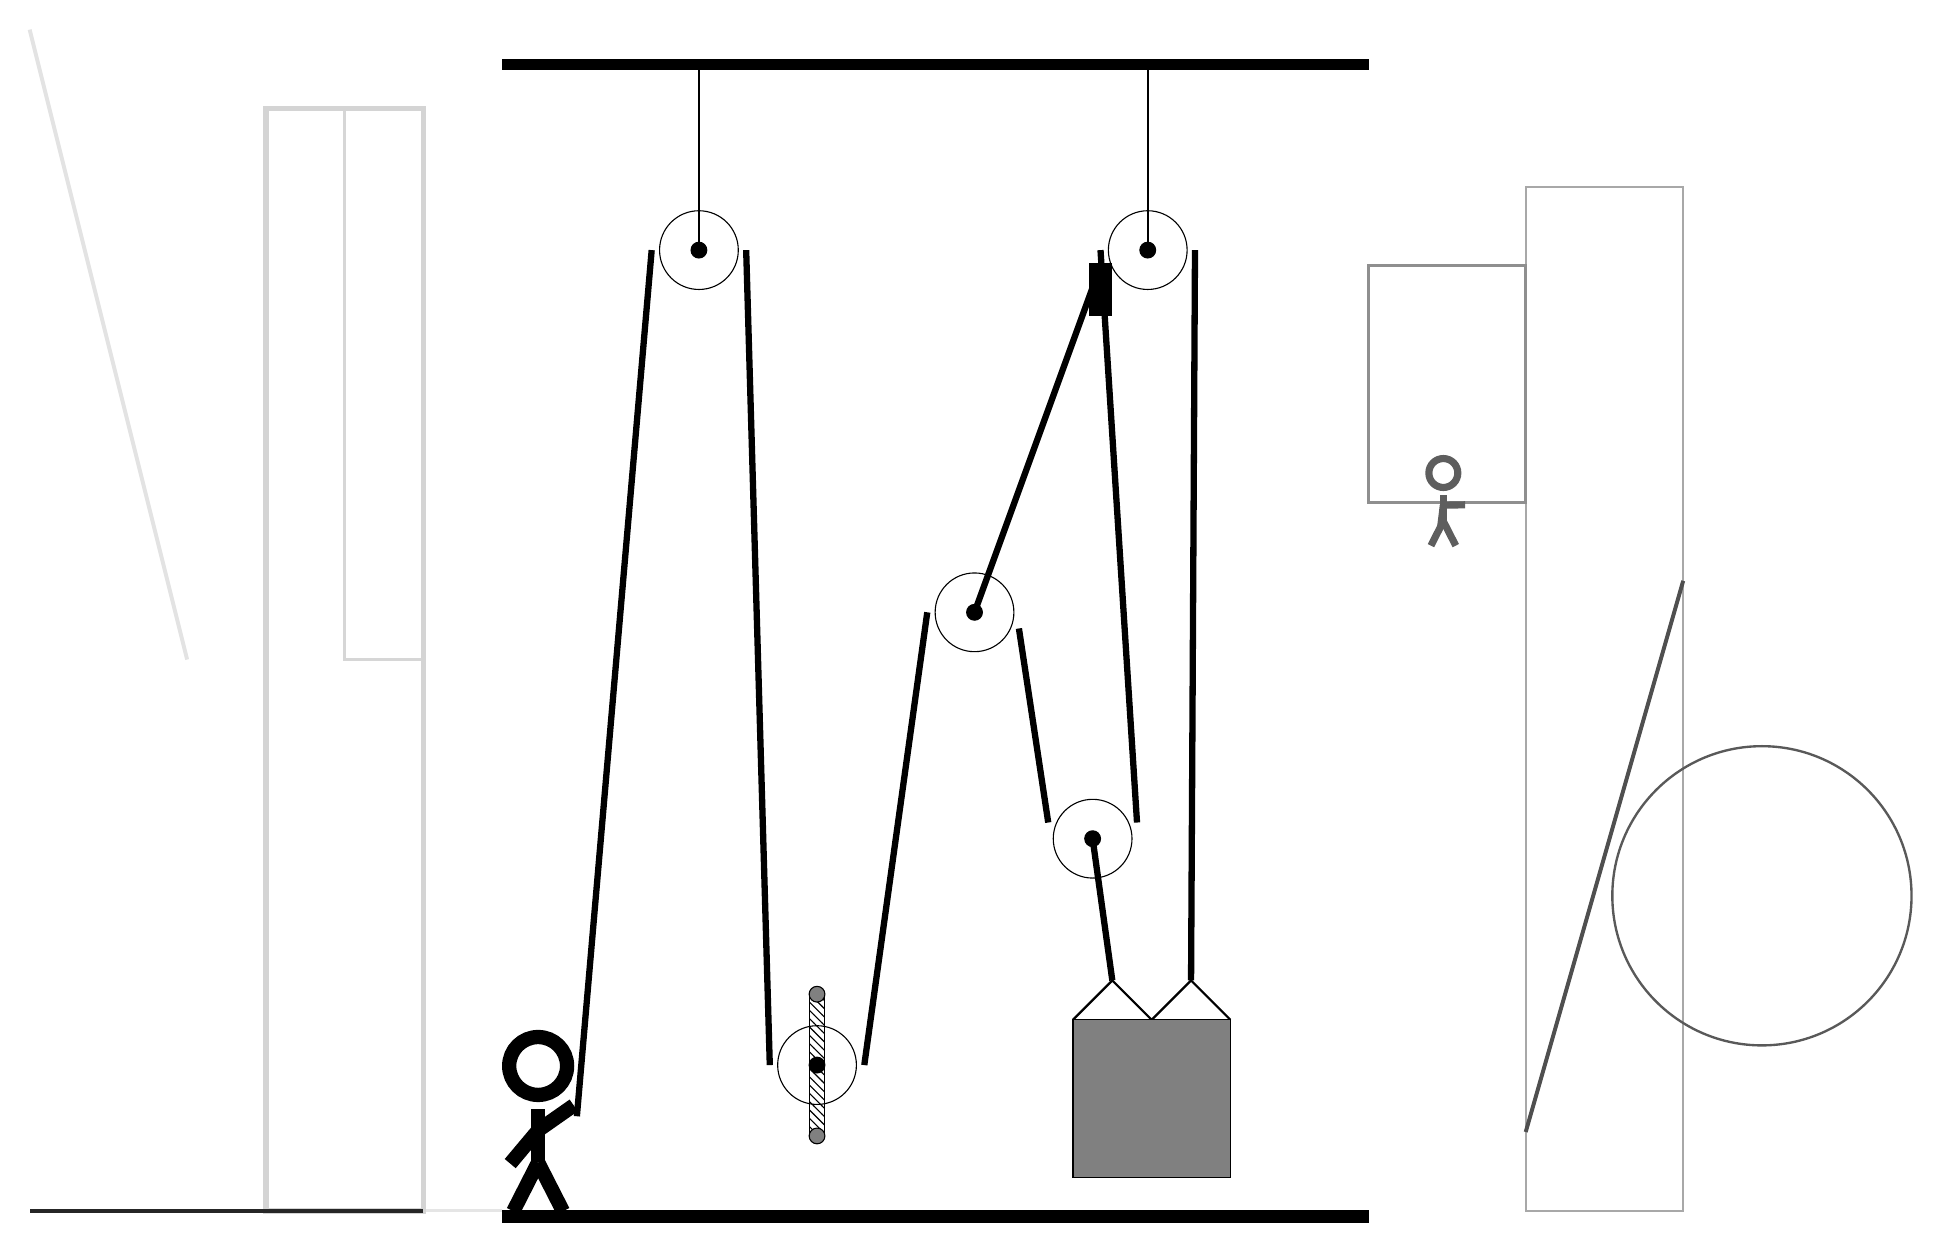
\begin{tikzpicture}
			%%%%% START %%%%%
			
			\draw[fill=black] (-6, 11.5) rectangle (5, 11.625);
			
			\draw (0, 4.6) circle (0.5);
			\draw[fill=black] (0, 4.6) circle (0.1);
			
			\draw (1.5, 1.725) circle (0.5);
			\draw[fill=black] (1.5, 1.725) circle (0.1);
			
			\draw (2.2, 9.2) circle (0.5);
			\draw[fill=black] (2.2, 9.2) circle (0.1);
			\draw[thick] (2.2, 9.2) -- (2.2, 11.5);
			
			\draw[line width=0.3mm, color=black!34] (7, -3) rectangle (9, 10);
			
			\draw[line width=0.4mm, color=black!16] (-8, 4) rectangle (-7, 11);
			\draw[line width=0.4mm, color=black!10] (-6, -3) rectangle (-9, -3);
			\draw[line width=0.4mm, color=black!44] (5, 6) rectangle (7, 9);
			\draw[line width=0.7mm, color=black!17] (-7, 11) rectangle (-9, -3);
			\draw[line width=0.5mm, color=black!11](-10, 4) -- (-12, 12);
			
			\draw [line width=0.3mm, color=black!65](10, 1) circle (1.9);
			\draw[line width=0.5mm, color=black!85](-7, -3) -- (-12, -3);
			\draw[line width=0.5mm, color=black!69](7, -2) -- (9, 5);
			\node[line width=0.4mm, color=black!63] at (6, 6) {\Strichmaxerl[5][83][1]};
			
			\draw (-3.5, 9.2) circle (0.5);
			\draw[fill=black] (-3.5, 9.2) circle (0.1);
			\draw[thick] (-3.5, 9.2) -- (-3.5, 11.5);
			
			\draw (-2, -1.15) circle (0.5);
			\draw[fill=black] (-2, -1.15) circle (0.1);
			\draw[pattern=north west lines, pattern color=black] (-2.1, -0.25) rectangle (-1.9, -2.05);
			\draw[fill=black!50] (-2, -0.25) circle (0.1);
			\draw[fill=black!50] (-2, -2.05) circle (0.1);
			
			\draw[thick]  (1.25, -0.575) -- (1.75, -0.075) -- (2.25, -0.575) -- (2.75, -0.075) -- (3.25, -0.575);
			\draw[fill=black!50] (1.25, -0.575) rectangle (3.25, -2.575);
			\draw[line width=0.8mm] (-5.05, -1.8) -- (-4.1, 9.2);
			\centerarc[line width=0.8mm](-3.5, 9.2)(0:180:0.6);
			\draw[line width=0.8mm] (-2.9, 9.2) -- (-2.6, -1.15);
			\centerarc[line width=0.8mm](-2, -1.15)(180:360:0.6);
			\draw[line width=0.8mm] (-1.4, -1.15) -- (-0.6, 4.6);
			\draw[line width=0.8mm] (0, 4.6) -- (1.6, 9.0);
			\draw[line width=0.8mm, fill=black](1.5, 8.4) rectangle (1.7, 9.0);
			\centerarc[line width=0.8mm](0, 4.6)(-20:180:0.6);
			\draw[line width=0.8mm] (0.5638, 4.3948) -- (0.9362, 1.9302);
			
			\centerarc[line width=0.8mm](1.5, 1.725)(160:380:0.6);
			\draw[line width=0.8mm] (2.0638, 1.9302) -- (1.6, 9.2);
			\draw[line width=0.8mm](1.5, 1.725) -- (1.75, -0.075);
			\centerarc[line width=0.8mm](2.2, 9.2)(0:180:0.6);
			\draw[line width=0.8mm] (2.8, 9.2) -- (2.75, -0.075);
			
			\node at (-5.5, -1.9) {\Strichmaxerl[10][50][35]};
			
			\draw[fill=black] (-6, -3) rectangle (5, -3.15);
			
			%%%%% END %%%%%
		\end{tikzpicture}
	\end{figure}	
\end{document}